\mode<all>
% Incluyo los paquetes necesarios.
% para no tener problemas con acentos etc.
\usepackage[utf8]{inputenc}
% en español
\usepackage[spanish]{babel}
%matemática
\usepackage{amsmath}
% este no se si hace falta pero por las dudas
\usepackage{graphicx}
% para incluir peliculas
\usepackage{multimedia}
% para usar segunda pantalla
\usepackage{pgfpages}
\usepackage{pgf}
% para hacer dibujitos
\usepackage{tikz}
\usetikzlibrary[automata,calc,arrows,decorations.pathmorphing,backgrounds,shapes,
patterns,positioning,fit,petri,overlay-beamer-styles]
\tikzstyle{every picture}+=[remember picture]
%recuadros sencillos
%\usepackage{tcolorbox}
% enumeradores intercambiables
\usepackage{enumerate}
% para subtitulos en figuras
\usepackage{subcaption}
%listings for code input
\usepackage{listings}
%verbatim input from file!
\usepackage{verbatim}
\usepackage{fancyvrb}
% para modificar los encabezados y pies de página.
%\usepackage{fancyhdr}
%\pagestyle{fancy}
\usepackage{standalone}

\definecolor{codegreen}{rgb}{0,0.6,0}
\definecolor{codegray}{rgb}{0.5,0.5,0.5}
\definecolor{codepurple}{rgb}{0.58,0,0.82}
%\definecolor{backcolour}{rgb}{0.95,0.95,0.0.1}

\lstset{
    basicstyle=\fontsize{8}{10}\selectfont\ttfamily, 
    backgroundcolor=\color{Beige},   
    frame=lines,
    commentstyle=\color{codegreen},
    keywordstyle=\color{magenta},
    numberstyle=\tiny\color{codegray},
    stringstyle=\color{codepurple},
    breakatwhitespace=false,         
    breaklines=true,                 
    captionpos=b,                    
    keepspaces=true,                 
    numbers=left,                    
    numbersep=5pt,                  
    showspaces=false,                
    showstringspaces=false,
    showtabs=false,                  
    tabsize=4
}



%\mode<presentation>{
% para ver las notas con la presentacion.  
%\setbeameroption{hide notes}
%para dejar las notas en la segunda patnalla
%}

% incluyo los beamercolors
%%%%%%%%%% BEAMERCOLORS
% el recuadro para el titulo
\setbeamercolor{title}{fg=white,bg=Purple}
% el recuadro para el subtitulo
\setbeamercolor{subtitle}{fg=white,bg=DarkOliveGreen}
% los títulos de las secciones tienen su colorinche:
\setbeamercolor{sectionbox}{fg=white,bg=Purple}
% cada diapositiva tendrá su color de título.
\setbeamercolor{frametitle}{fg=white,bg=ForestGreen}
% el título de las secciones tienen también su color. 
\setbeamercolor{sectiontitle}{fg=white,bg=violet}

%%%% CUSTOM BEAMERCOLORS
% estos cuadros los defino para ubicar al lector en los temas que se tratan
% son los cuadritos que aparecen arriba del título. 
\setbeamercolor{structure0}{fg=white,bg=gray}
\setbeamercolor{structure1}{fg=black,bg=DarkGray}
\setbeamercolor{structure2}{fg=black,bg=lightgray}
% defino un cuadro para usar en alguna oportunidad, creo que para titulos. 
\setbeamercolor{whitebox}{fg=black,bg=white}
% un cuadro para resaltar
\setbeamercolor{highlight1}{fg=black,bg=Gold}

% beamer colors for headers and etc.
\setbeamercolor{header1}{fg=white,bg=Blue}
\setbeamercolor{header2}{fg=black,bg=Red}
\setbeamercolor{header3}{fg=black,bg=ForestGreen}

%code block
\setbeamercolor{codeblock}{fg=Blue, bg=Beige}
\setbeamerfont{codeblock}{family=\ttfamily,size=\scriptsize}


%incluyo el tema y modificaciones
%%% BEAMER THEME
% el tema 'boxes' es igual al default pero permite definir boxes de estructura 
% a mano. 
\mode<presentation>{
  \usetheme{boxes}
  % los boxes que identifican lo que se esta leyendo
    % box de la izquierda: la materia (subtitulo)
    \addheadbox{structure2}{\quad \tiny \insertshortsubtitle}
  %  box del medio en cabecera, el titulo de la clase
    \addheadbox{structure0}{\quad \tiny  \inserttitle \quad } 
  % box en a la derecha , eltítulo de la sección. 
    \addheadbox{structure1}{\quad \tiny \insertsection}
}
% tema interno y de colores para las diapositivas normales. 
\useinnertheme{rectangles}
\usecolortheme{dove}
% la fuente de las ecuaciones
\usefonttheme[onlymath]{serif}

% entorno codeblock para meter piezas de código.
% el color se definió en BEAMERCOLORS

\newenvironment{codeblock}
{
  \begin{beamercolorbox}{codeblock}
    \usebeamerfont{codeblock}
}
{
  \end{beamercolorbox}
}



% modifico los temas
  \titlegraphic{%
\includegraphics[width=0.25\textwidth]{./PREAMBLE/logo-isabt25.png}
                
\includegraphics[width=0.25\textwidth]{./PREAMBLE/logo-isabato.png}
  		\hfill
		
\includegraphics[width=0.25\textwidth]{./PREAMBLE/ISOLOGOCNEA.png}
		\hfill
  		
\includegraphics[width=0.25\textwidth]{./PREAMBLE/unsam-horizontal.png}}

\mode<presentation>{
\setbeamertemplate{title page}[center]
{
  %
\includegraphics[width=0.25\textwidth]{./PREAMBLE/ISOLOGOCNEA.png}
  \inserttitle
  \insertsubtitle
  \insertauthor
  \insertinstitute
%  \inserttitlegraphic
}
}


% defino el template para las dapositivas con los titulos de las secciones. 
%es una recetita que saqué de algun lado. 
\setbeamertemplate{section page}{
  \begin{beamercolorbox}[ht=5ex,dp=1ex,wd=\paperwidth,center]{sectionbox}
    \begin{centering}
     \usebeamerfont{section  title} \insertsection 
    \end{centering}
  \end{beamercolorbox}
}
\AtBeginSection[]{
  \begin{frame}[plain]
    \begin{center}
    \quad \inserttitle \quad  
    \end{center}
    \sectionpage
  \end{frame}
}

% remover los simbolos de navegacion
% porque sacan espacio 
\mode<presentation>{
\setbeamertemplate{navigation symbols}{}
\setbeamertemplate{footline}[page number]
% me gustan los titulos a la derecha
\setbeamertemplate{frametitle}[default][right]%{
}
\mode<handout>{
 \setbeamertemplate{headline}{}
 \setbeamertemplate{frametitle}{}
 \setbeamertemplate{background}{
   \tikz\node [rectangle,minimum width=0.995\paperwidth,
   minimum height=0.995\paperheight,draw,anchor=south west,
   line width=2pt]  {};
 }
 \setbeamertemplate{footline}{}
}
% aparentemente el siguiente beamertemplate
%se ejecuta en modo artículo. habría que ver
%la forma de sacale probecho. 
% notar que vale solo para las framesque se incluyen 
% directamente en el artículo y no vale para 
% \includeslide.
% \setbeamertemplate{frame begin}
% \setbeamertemplate{frame end}


% no se si es el mejor lugar para definirlo, 
% pero las \includeslides deben quedar fijas al
% tamaño de la página:

%\mode<article>{
%\renewcommand\includeslide[1]{
%  \includeslide[width=\textwidth]{#1}
%}
%}

% defino el template para la diapositiva del título

%%%%%%%%%%%%%%%%%%%%%%%%%%%%%%%%
% Defino la Clase
%%%%%%%%%%%%%%%%%%%%%%%%%%%%%%%%
\subtitle[Modelización 2020]{ Modelización de Propiedades y Procesos 2021 }
\author{Ruben Weht\inst{1,2} \and Mariano Forti\inst{1,3} }
\institute{
%  \inst{1}Instituto de Tecnología Prof. Jorge Sabato
%  \and
  \inst{1}Fisica del Sólido, Edificio TANDAR, \url{weht@cnea.gov.ar},
  interno 7104
  \and
  \inst{2}División Aleaciones Especiales, Edificio 47 (microscopía),
  \url{mforti@cnea.gov.ar}, interno 7832
}

\mode<presentation>{\date{}}

\mode<article>{
  \date{
    \small
%  \textsuperscript{1} Instituto de Tecnología Prof. Jorge Sabato\\
  \textsuperscript{1}Fisica del Sólido, Edificio TANDAR, \url{weht@cnea.gov.ar},
  interno 7104 \\
  \textsuperscript{2}División Aleaciones Especiales, Edificio 47 (microscopía),
  \url{mforti@cnea.gov.ar}, interno 7832
}

%defino los encabezados y pies de págna para
% dodo el documento en función de la materia y la
% clase.
%\fancyhead[L]{\tiny Modelización de Materiales 2019}
%\fancyhead[R]{\tiny \leftmark}
}

\title{
  \mode<article>{
% 
\includegraphics[height=1cm]{./PREAMBLE/logo-isabt25.png}

\includegraphics[height=1cm]{./PREAMBLE/Beninson.jpeg}
\hfill

\includegraphics[height=1cm]{./PREAMBLE/ISOLOGOCNEA.png}
\hfill
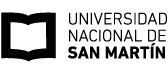
\includegraphics[height=1cm]{./PREAMBLE/logo-unsam.png}
\\}  Apéndice: Instalación de Python más fácil que nunca}
\subject{Apéndice: Instalación de Python más fácil que nunca}
\keywords{Python, Modelizacion 2021, Programación}
%linea para fbox
\setlength\fboxsep{0pt}
\setlength\fboxrule{5pt}
% Inicia el documento.
\begin{document}

% Título de la clase. 
\mode<presentation>{
\begin{frame}[plain]
\titlepage
\end{frame}
}

%\mode<article>{
%\maketitle
%}

\begin{frame}<presentation>[label=FrameWinPython]
  \frametitle{https://winpython.github.io/}
  \center
  \href{https://winpython.github.io/}{ 
  \includegraphics[width=0.5\textwidth]{winpython_title.png}
  }

  \includegraphics[width=\textwidth]{winpython_launchers.png}

  \href{https://sourceforge.net/projects/winpython/files/latest/download}{Descargar últuma version desde SourceForge}

  \tiny https://sourceforge.net/projects/winpython/files/latest/download
\end{frame}

\begin{frame}<presentation>[label=FrameEsperar]
  \frametitle{Esperar}
\center
  \includegraphics[height=0.9\textheight]{mate.jpg}

\end{frame}

\begin{frame}<presentation>[label=FrameExctract]
  \frametitle{Extraer Archivos}
 

  \begin{tikzpicture}
    \node<1-> {\fbox{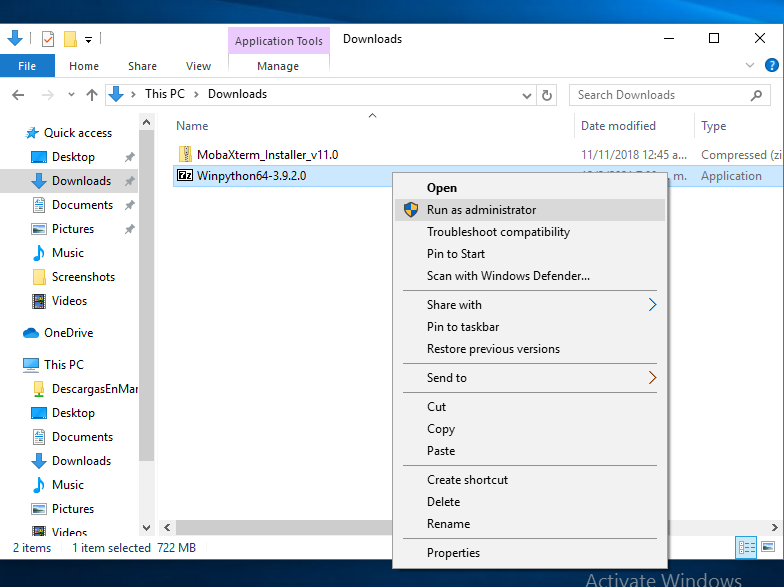
\includegraphics[width=0.5\textwidth]{Screenshots/RunAsAdministrator.png}}};

    \node<2-> at (3,0) {\fbox{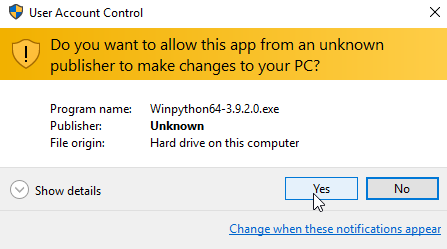
\includegraphics[width=0.5\textwidth]{Screenshots/GiveAccess.png}}};

    \node<3-> at (7,-1) {\fbox{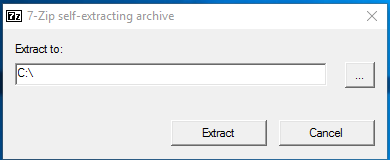
\includegraphics[width=0.5\textwidth]{Screenshots/ChangePath.png}}};

  \end{tikzpicture}

\end{frame}

\begin{frame}<presentation>[label=FrameEsperarII]
  \frametitle{Esperar (II)}
\center
  \href{https://www.youtube.com/playlist?list=PLQkH8HQf-uqoNlgHH9g0eBzeIQbvKiilH}{
    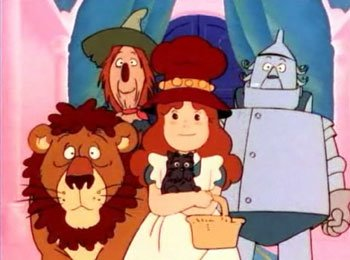
\includegraphics[height=\textheight]{oz-no-mahotsukai-episode-17_521.png}
  }
\end{frame}

\section{Probar}
\begin{frame}<presentation>[label=FrameProbar]
  \frametitle{Probamos}

  \begin{tikzpicture}
    \node<1-> at (0,0) {\fbox{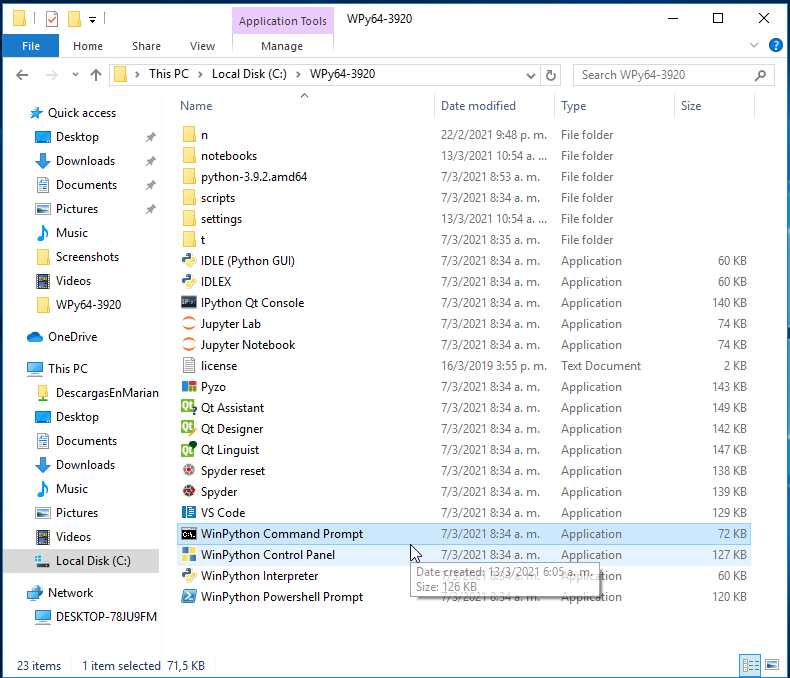
\includegraphics[width=0.5\textwidth]{Screenshots/PythonPrompt.png}}};

    \node<2-> at (3,-1) {\fbox{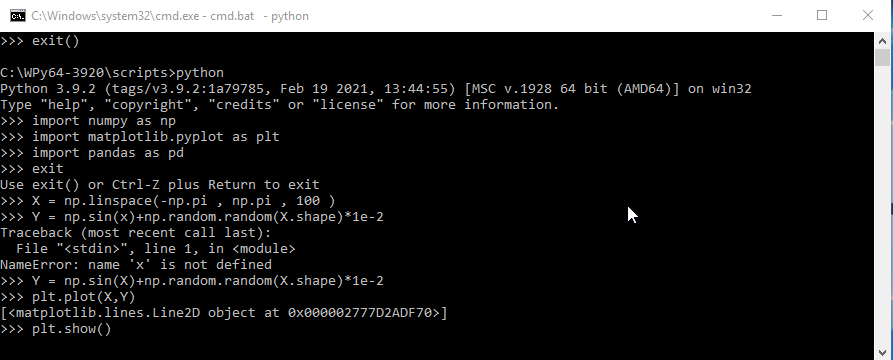
\includegraphics[width=0.5\textwidth]{Screenshots/JugamosUnRato.png}}};

    \node<3-> at (6,-1) {\fbox{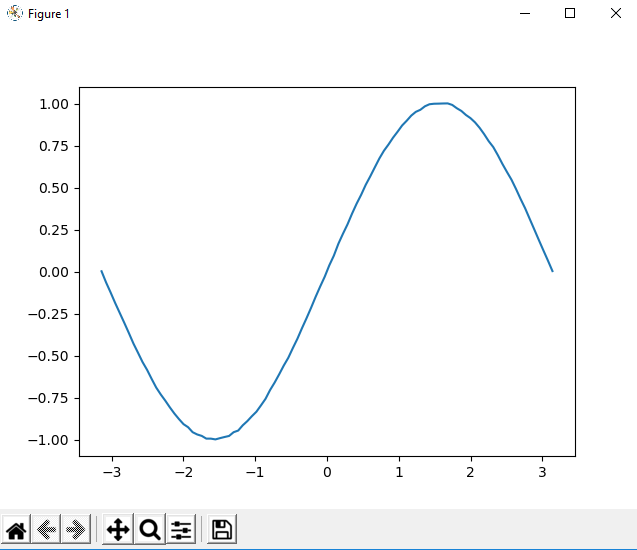
\includegraphics[width=0.5\textwidth]{Screenshots/UnGrafico.png}}};

  \end{tikzpicture}


\end{frame}

\section{Configuracion}

\begin{frame}<presentation>[label=FrameConfigurar]
  \frametitle{Mínima configuracion}

  \begin{tikzpicture}

    \node at (0,0) {\fbox{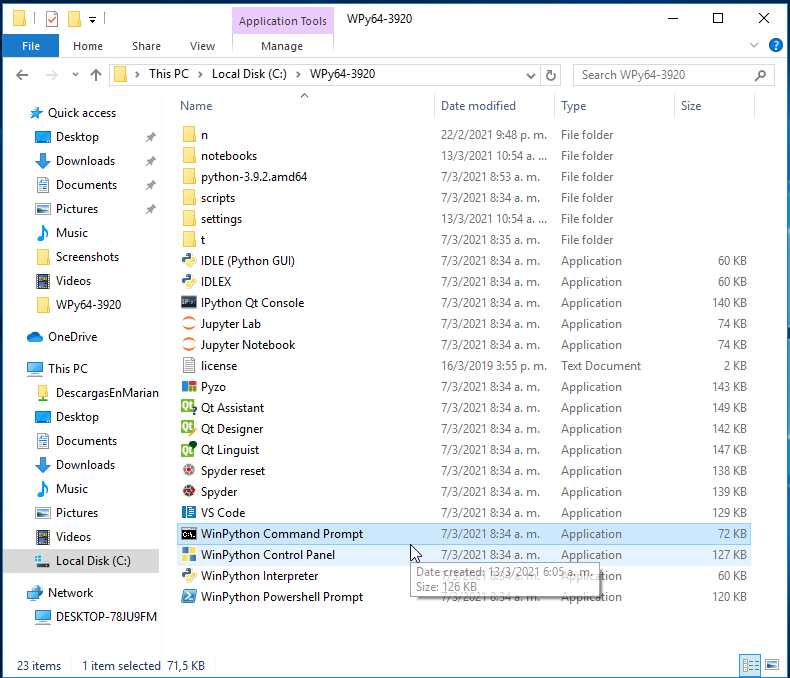
\includegraphics[width=0.5\textwidth]{Screenshots/PythonPrompt.png}}};

    \node at (5,0) {\fbox{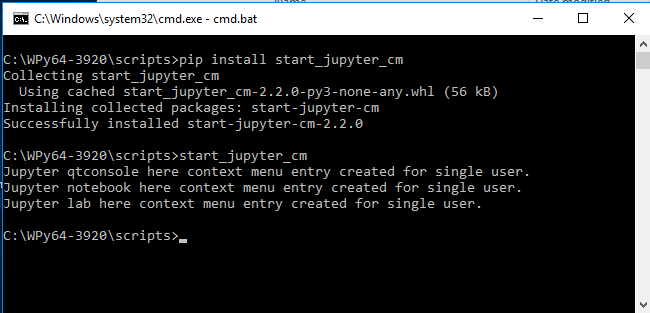
\includegraphics[width=0.6\textwidth]{Screenshots/Configurar.png}}};

  \end{tikzpicture}
\end{frame}

\section{Usamos Jupyter Lab}

\begin{frame}<presentation>[label=FrameJupyterLab]
  \frametitle{Abrimos Jupyter Lab desde una carpeta}

  \center

  \begin{columns}
    \column{0.6\textwidth}
    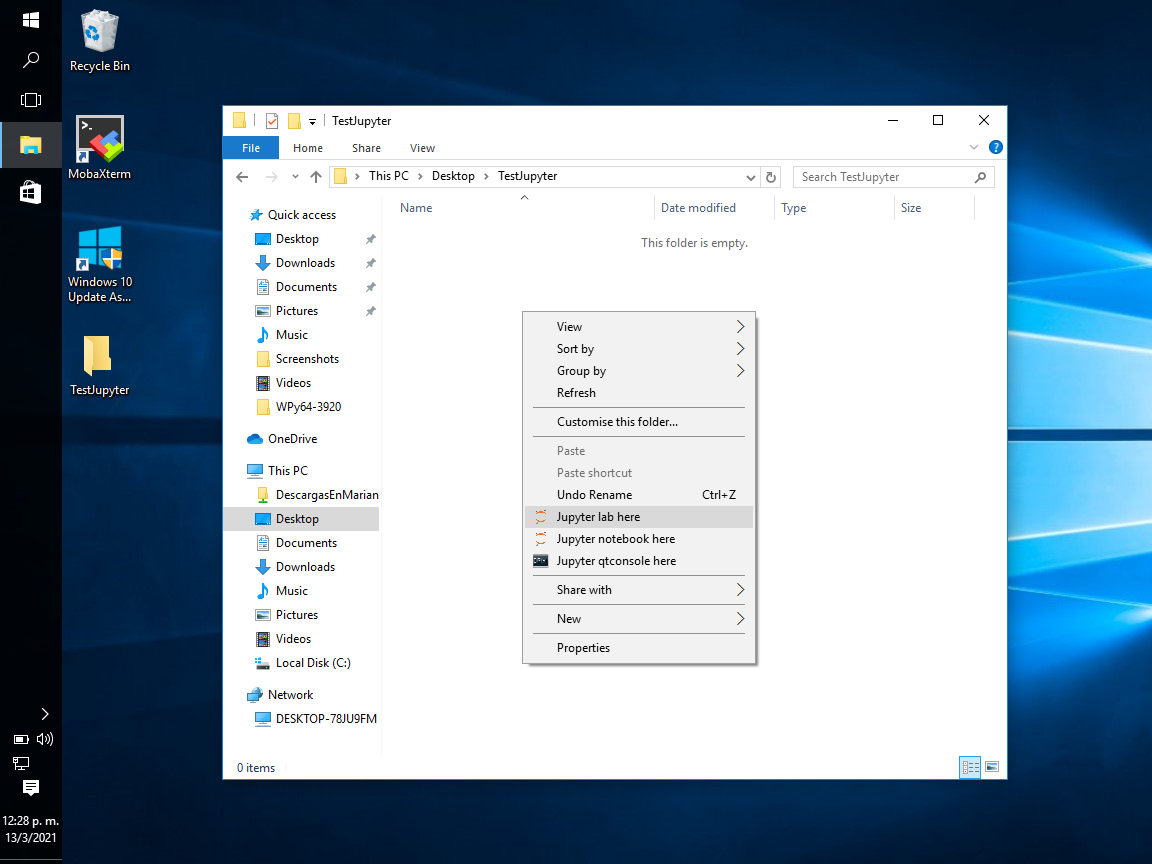
\includegraphics[height=0.7\textheight]{Screenshots/ClickIzquierdo.png}
    \column{0.4\textwidth}

    \begin{itemize}
	\item Creamos una carpeta de trabajo y navegamos hasta allí

	\item click izquierdo
	
	\item click en \emph{Jupyter Lab Here}

    \end{itemize}

  \end{columns}
\end{frame}

\begin{frame}<presentation>[label=FrameEnjoy]
  \frametitle{¡A trabajar !}

  \center
  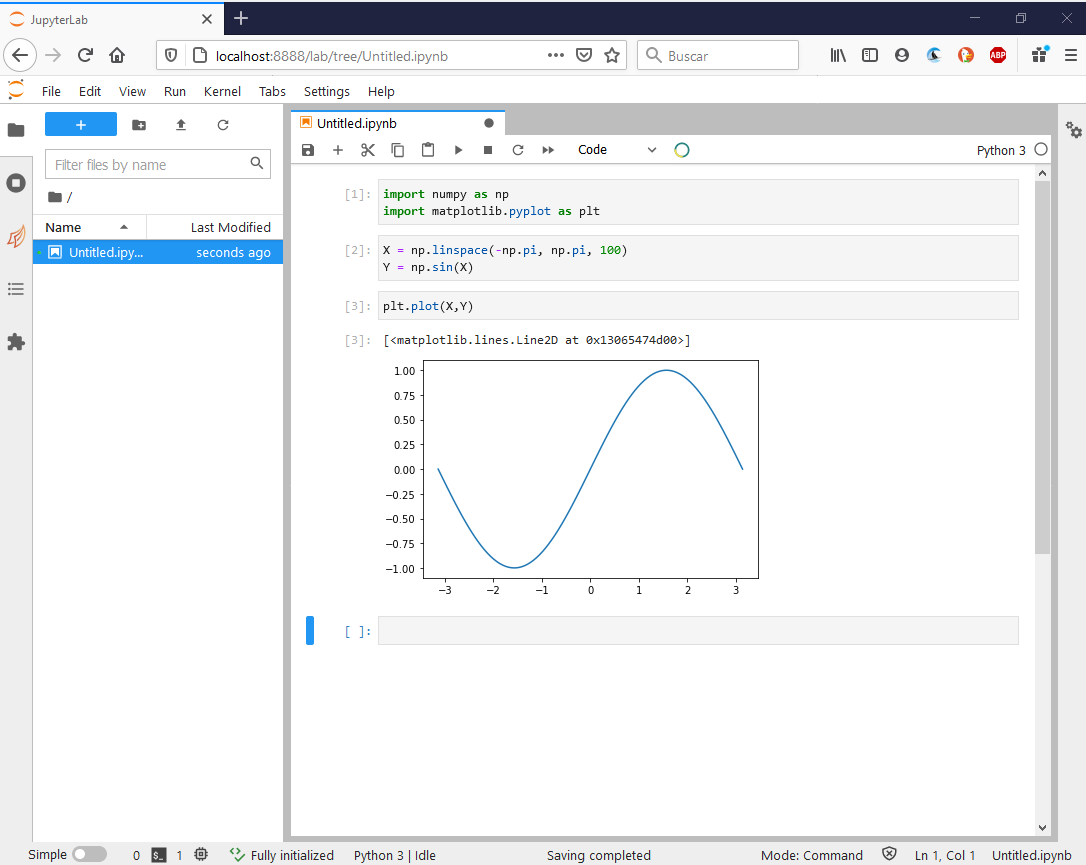
\includegraphics[width=0.6\textwidth]{Screenshots/PlayHappy.png}

\end{frame}

\end{document}
